\begin{figure}[!htp]
    \centering
    \caption{Out-of-sample fit of the model}
    \label{fig:out_sample_fit}
    \begin{subfigure}[b]{0.49\textwidth}
        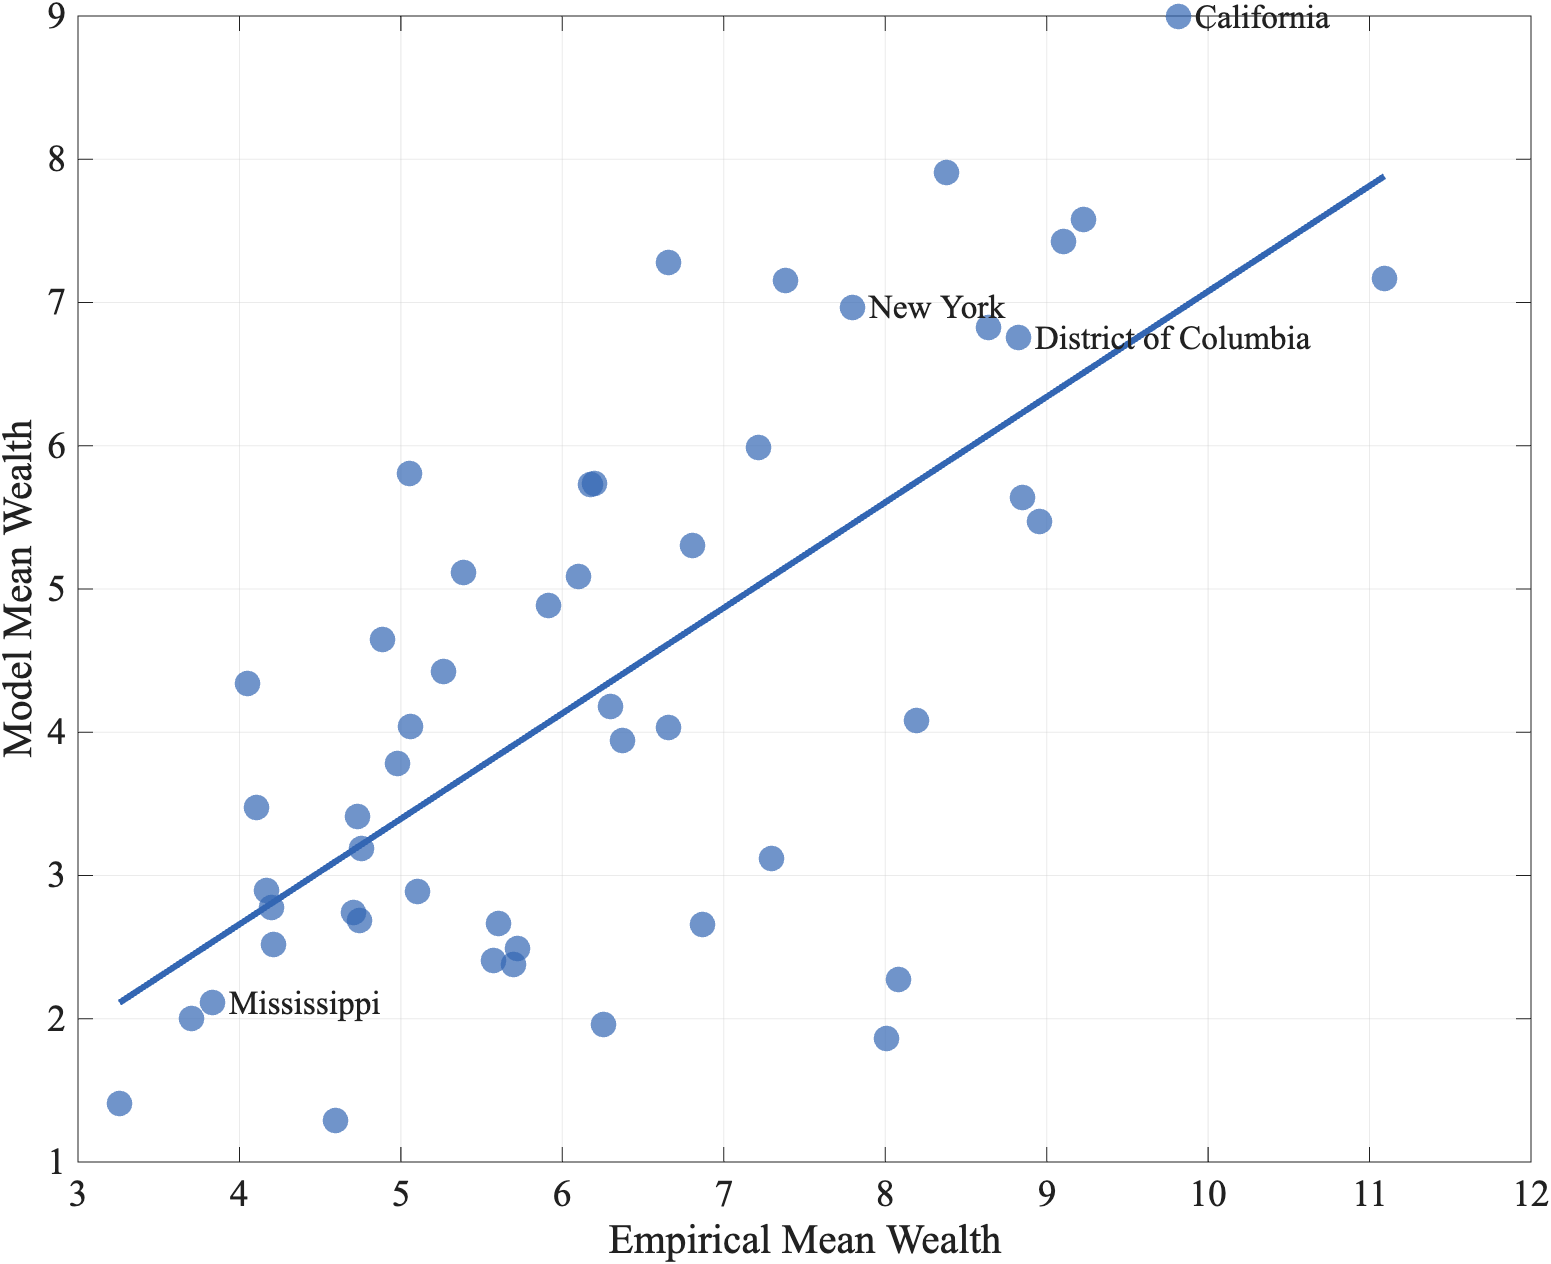
\includegraphics[width=\textwidth]{../Output/graph_comparison/out_sample_fit/out_sample_fit_model_mean_wealth.png}
        \caption{Wealth Comparisons}
        \label{fig:out_sample_wealth}
    \end{subfigure}
    \hfill
    \begin{subfigure}[b]{0.49\textwidth}
        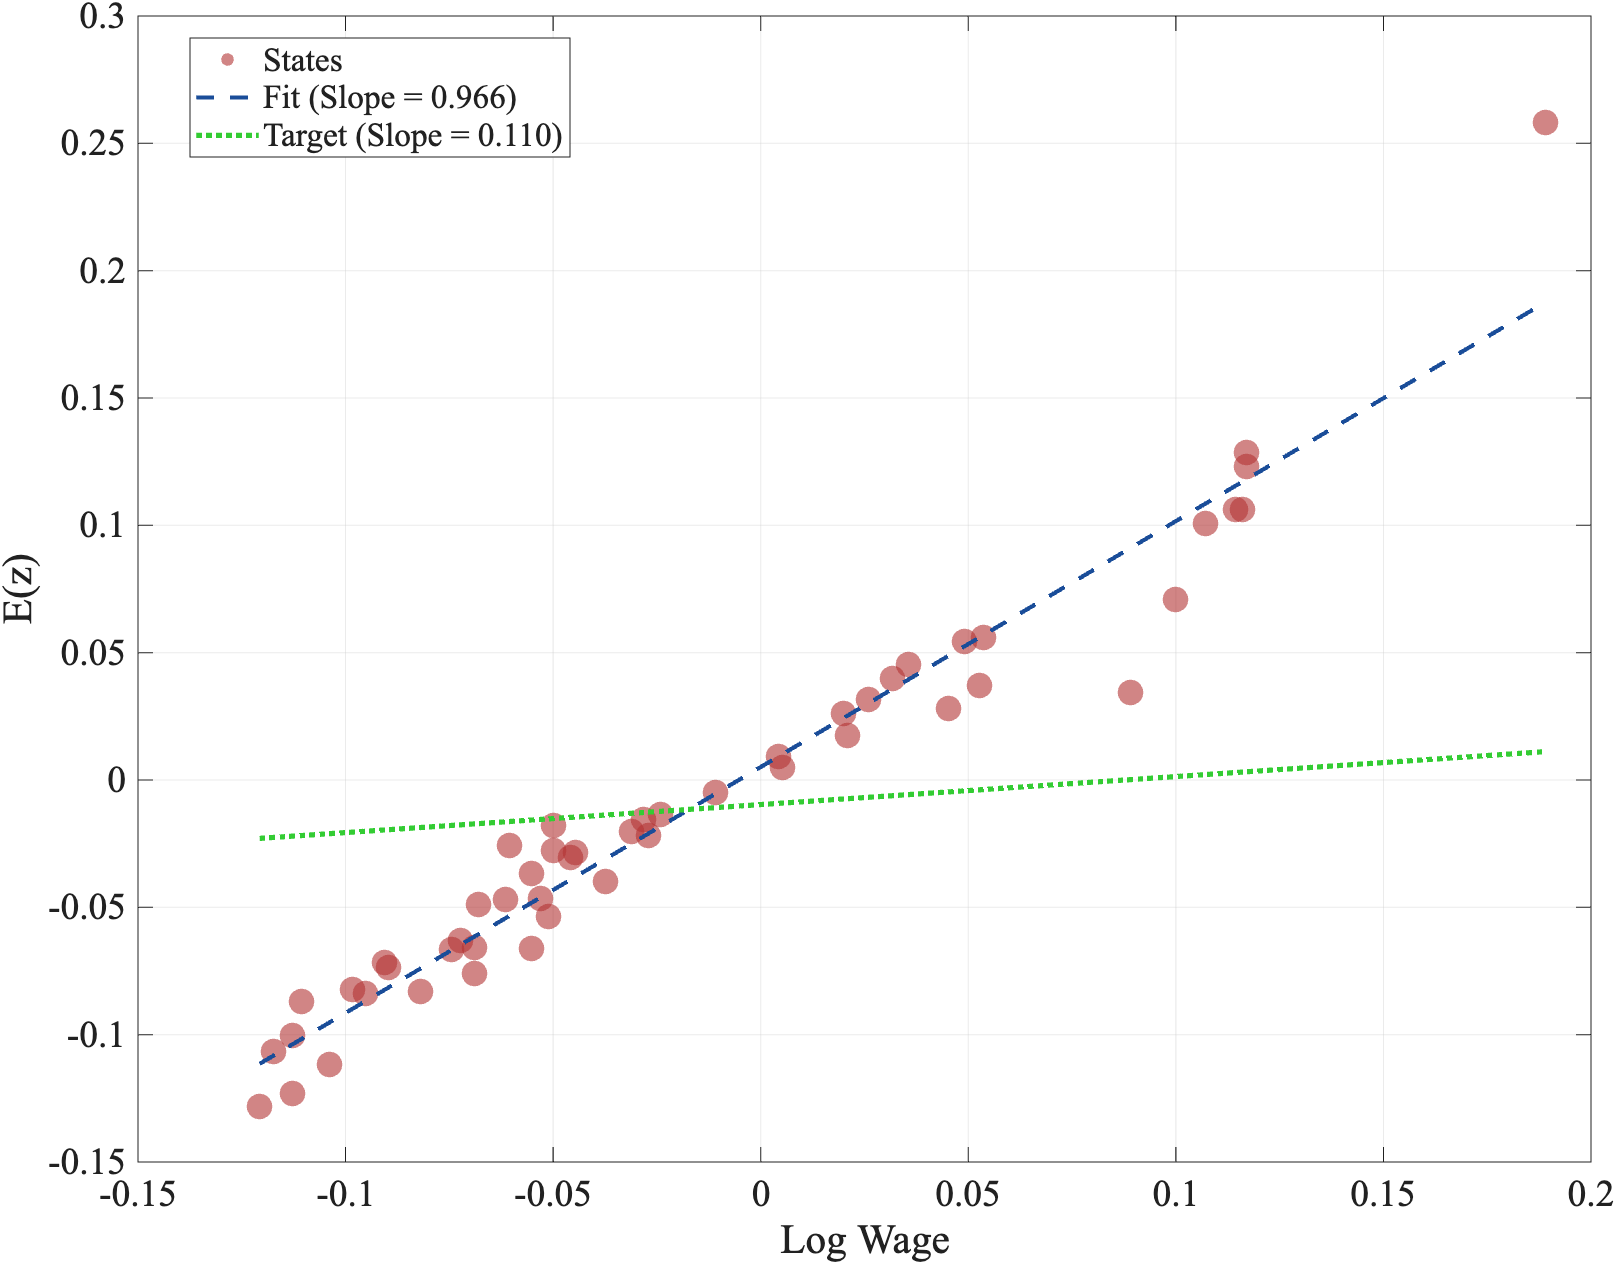
\includegraphics[width=\textwidth]{../Output/graph_comparison/out_sample_fit/out_sample_fit_e_z.png}
        \caption{Migration Sorting}
        \label{fig:out_sample_sorting}
    \end{subfigure}
    
    \vspace{1em}
    \begin{subfigure}[b]{0.49\textwidth}
        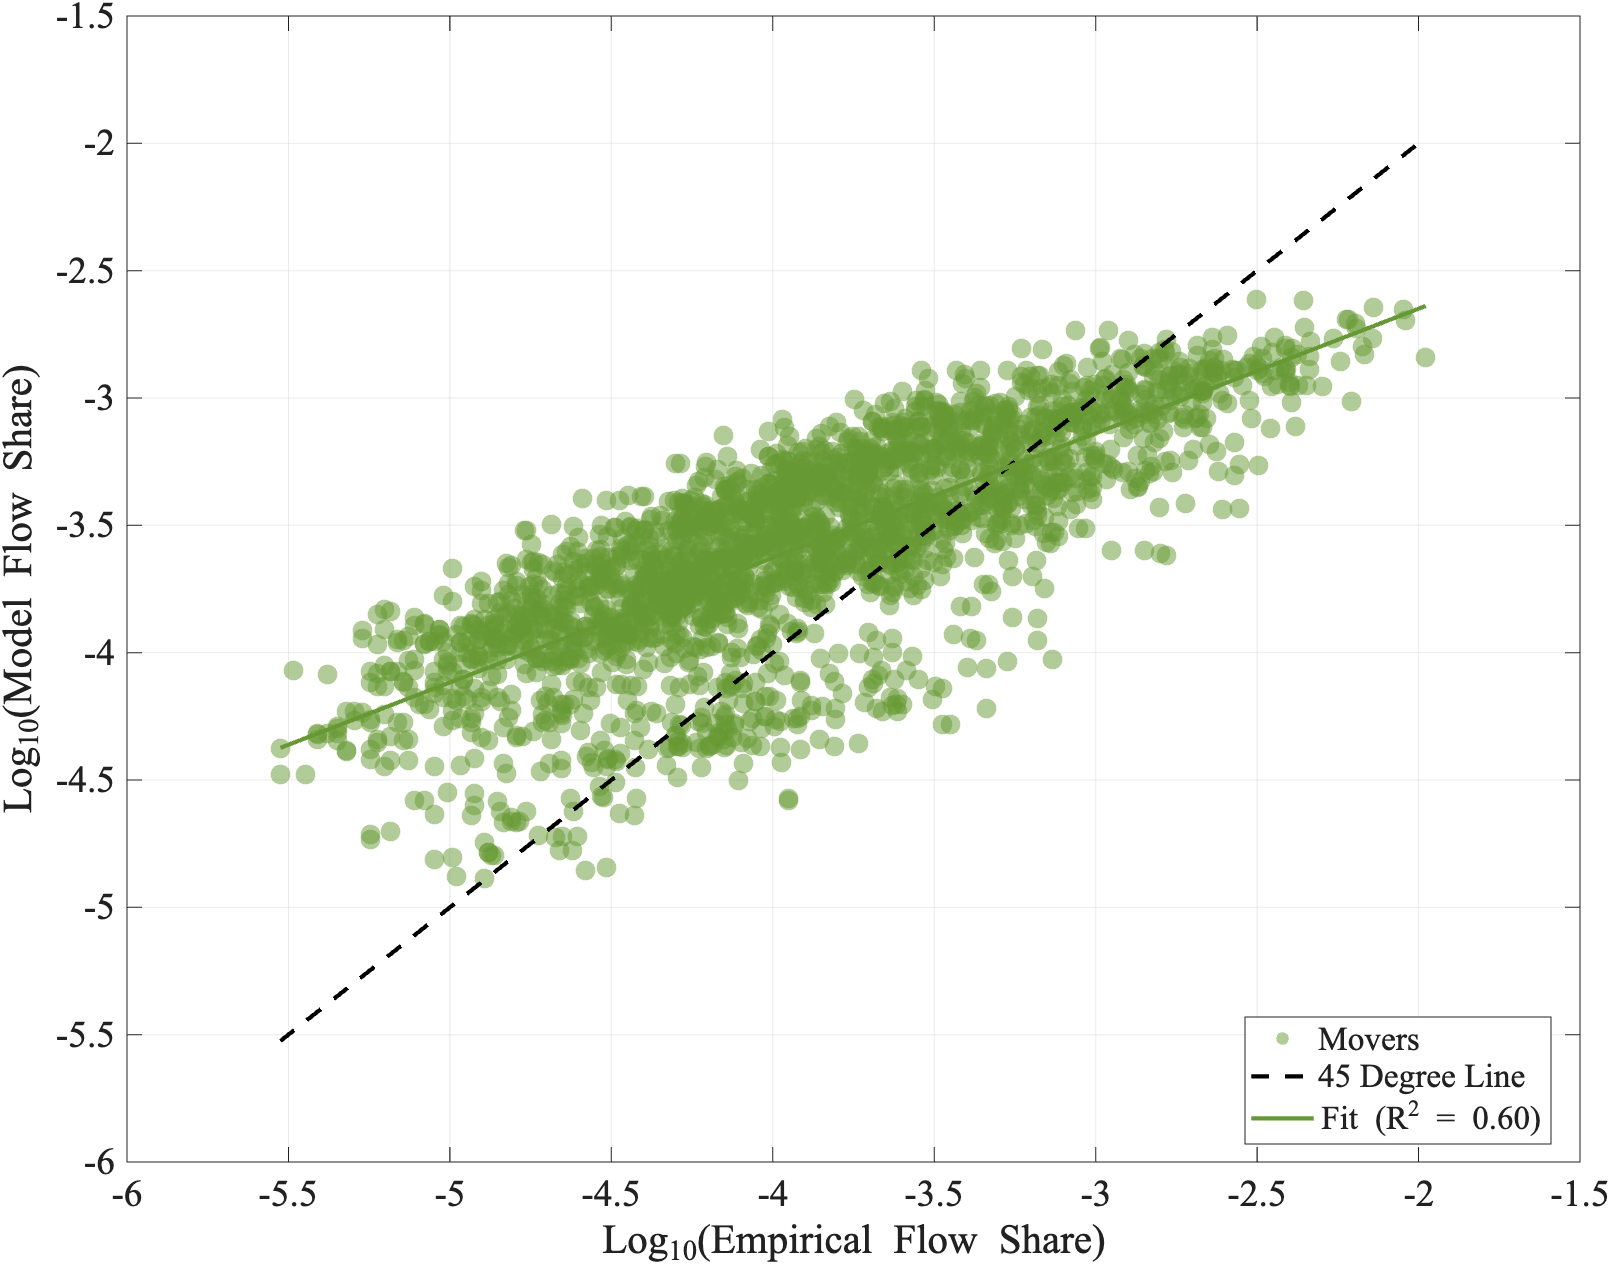
\includegraphics[width=\textwidth]{../Output/graph_comparison/out_sample_fit/out_sample_fit_log_10_model_flow_share.png}
        \caption{Bilateral Migration Flows}
        \label{fig:out_sample_flows}
    \end{subfigure}
    
    \begin{minipage}{\textwidth} \vspace{0.5em}
      \footnotesize{\textbf{Note:} Out-of-sample fit of the model along three dimensions: (a) average state-level wealth, (b) spatial sorting of productive workers across states, and (c) bilateral migration flows (in log shares) between states. In panel (a), the black line displays the OLS regression of model-implied mean wealth on empirical values from Geowealth-US 2010. In panel (b), the regression of expected productivity $E(z)$ on log wages (blue dashed line) tracks the slope of $0.11$ (green dotted line) from \cite{dvorkin_geography_2025}. In panel (c), the OLS regression of model-implied bilateral log migration shares on empirical values from the ACS 2010-2019 is shown.}
    \end{minipage}
\end{figure}
